% !tex root=./main.tex

\vspace*{-1ex}
\section{EXPERIMENTS}
\vspace*{-1ex}
\label{sec:experiments}

% Purpose of experiments
% - run rws and iwae on something else than MNIST
% - compare rws to all other methods
% - confirm tighter is not necessarily better and effect on generative model
% - gradient estimator of ww is lower variance than that of iwae
% - mode collapse of ww, check if defensive rws helps
% - badness of ws
% - revisiting competitiveness of rws on large models
% - check whether claims hold for continuous

The \gls{IWAE} and \gls{RWS} algorithms have primarily been applied to problems with continuous latent variables and/or discrete latent variables that do not actually induce branching (such as sigmoid belief networks;~\cite{neal1992connectionist}).
%
The purpose of the following experiments is to compare \gls{RWS} to \gls{IWAE} combined with control variates and continuous relaxations (c.f \cref{sec:method}) on models with conditional branching, and show that it outperform such methods.
%
We empirically demonstrate that increasing the number of particles $K$ can be detrimental in \gls{IWAE} but advantageous in \gls{RWS}, as evidenced by achieved \glspl{ELBO} and average distance between true and amortized posteriors.
% \begin{compactitem}
%   \item , \label{experiment-point-1}
%   \item \gls{RWS} has a lower variance gradient estimator for $\phi$ than \gls{IWAE}, and
% \end{compactitem}
%

In the first experiment, we present learning and amortized inference in a \gls{PCFG}~\citep{booth1973applying}, an example \gls{SCFM} where continuous relaxations are inapplicable.
We demonstrate that \gls{RWS} outperforms \gls{IWAE} with a control variate both in terms of learning and inference.
The second experiment focuses on \glsreset{AIR}\gls{AIR}, the deep generative model of \cite{eslami2016attend}.
It demonstrates that \gls{RWS} leads to better learning of the generative model in a setting with both discrete and continuous latent variables, for modeling a complex visual data domain (c.f. \cref{sec:experiments/air}).
The final experiment involves a \gls{GMM} (\cref{sec:experiments/gmm}), thereby serving as a pedagogical example.
It explains the causes of why \gls{RWS} might be preferable to other methods in more detail.
\footnote{In \cref{app:sigmoid_belief_nets}, we include additional experiments on sigmoid belief networks which, however, are not \glspl{SCFM}.}

% The first experiment (\cref{sec:experiments/gmm}) aims to address all three points in a simple \gls{GMM} with a discrete latent variable used to select cluster locations.
% The next experiment, on \gls{AIR} (\cref{sec:experiments/air}), addresses the first point in a model containing both discrete latent variables used for branching as well as continuous latent variables in a more complex visual data domain.
% Finally, the \acrshort{MNIST} experiment (\cref{sec:experiments/mnist}) addresses the first point in a model with continuous latent variables.
%

% \todo{Didn't move this block to before ``Advantages of Reweighted Wake-Sleep'' because defensive \gls{RWS} is not introduced by then yet}
Notationally, the different variants of \gls{RWS} will be referred to as \gls{WS} and \gls{WW}.
The \emph{wake-phase $\theta$ update} is always used.
We refer to using it in conjunction with the \emph{sleep-phase $\phi$ update} as \acrshort{WS} and using it in conjunction with the \emph{wake-phase $\phi$ update} as \acrshort{WW}.
% %
% The variants differ in
% \begin{tabular}{@{}>{\bfseries}r@{\,\,}p{80ex}@{}}
%   \acrshort{WS} --  & using the \emph{sleep-phase $\phi$ update}, \\
%   \acrshort{WW} --  & using the \emph{wake-phase $\phi$ update}.
%   % \gls{WWS} -- & using both wake and sleep gradient estimators of $\phi$ where the
%   % gradient estimator is a uniform mixture of the two separate estimators.
% \end{tabular}
% %
Using both \emph{wake-} and \emph{sleep-phase $\phi$ updates} doubles the required stochastic sampling while yielding only minor improvements on the models we considered.
%
The number of particles $K$ used for the \emph{wake-phase $\theta$} and \emph{$\phi$ updates} is always specified, and computation between them is matched so
a \emph{wake-phase $\phi$ update} with batch size $B$ implies a \emph{sleep phase $\phi$ update} with $KB$ samples.

\subsection{PROBABILISTIC CONTEXT-FREE GRAMMAR}
\label{sec:experiments/pcfg}

% \begin{figure}
%   \includegraphics[width=\linewidth]{figures/pcfg/errors_end_points.pdf}
%   \caption{}
%   \label{fig:experiments/pcfg/astronomers_errors}
% \end{figure}
\begin{figure*}
  \centering
  % \includegraphics[width=0.94\textwidth]{figures/pcfg/errors.pdf}
  \includegraphics[width=\textwidth]{figures/pcfg/errors_vector.pdf}
  \vspace*{-0.7\baselineskip}
  \caption{
    \Gls{PCFG} training.
    \emph{(Top)}
    Quality of the generative model:
    While all methods have the same gradient update for $\theta$, the performance of \gls{WS} improves and is the best as $K$ is increased.
    Other methods, including \gls{WW}, do not yield significantly better model learning as $K$ is increased, since \gls{WS}'s inference network learns the fastest.
    \emph{(Bottom)}
    Quality of the inference network:
    \Gls{VIMCO} and \acrshort{REINFORCE} do not improve with increasing $K$.
    \Gls{WS} performs best as $K$ is increased, and while \gls{WW}'s performance improves, the improvement is not as significant.
    This can be attributed to the data-distribution bias being less significant than the bias coming from self-normalized \gls{IS} (c.f. \cref{sec:disadvantages}).
    Median and interquartile ranges from up to $10$ repeats shown (see text).
  }
  \label{fig:experiments/pcfg/astronomers_errors}
  \vspace*{-2ex}
\end{figure*}

% \begin{figure*}
%   \includegraphics[width=\textwidth]{figures/pcfg/both_errors.pdf}
%   \caption{}
%   \label{fig:experiments/pcfg/astronomers_errors}
% \end{figure*}

In this experiment we learn model parameters and amortize inference in a \gls{PCFG}~\citep{booth1973applying}.
Each discrete latent variable in a \gls{PCFG} chooses a particular child of a node in a tree.
Depending on each discrete choice, the generative model can lead to different future latent variables.
A \gls{PCFG} is an example of an \gls{SCFM} where continuous relaxations cannot be applied---weighing combinatorially many futures by a continuous relaxation is infeasible and doing so for futures which have infinite latent variables is impossible.

While supervised approaches have recently led to state-of-the-art performance in parsing~\citep{chen2014fast}, \glspl{PCFG} remain one of the key models for unsupervised parsing~\citep{manning1999foundations}.
Learning in a \gls{PCFG} is typically done via expectation-maximization~\citep{dempster1977maximum} which uses the inside-outside algorithm~\citep{lari1990estimation}.
Inference methods are based on dynamic programming~\citep{younger1967recognition,earley1970efficient} or search~\citep{klein2003parsing}.
Applying \gls{RWS} and \gls{IWAE} algorithms to \glspl{PCFG} allows learning from large unlabeled datasets through \gls{SGD} while inference amortization ensures linear-time parsing in the number of words in a sentence, at test-time.
Moreover, using the inference network as a proposal distribution in \gls{IS} provides asymptotically exact posteriors if parses are ambiguous.

% generative model
A \gls{PCFG} is defined by sets of terminals (or words) $\{t_i\}$, non-terminals $\{n_i\}$, production rules $\{n_i \to \zeta_j\}$ with $\zeta_j$ a sequence of terminals and non-terminals, probabilities for each production rule such that $\sum_j~P\left(n_i \!\to\! \zeta_j\right)~=~1$ for each $n_i$, and a start symbol $n_1$.
% A \gls{PCFG} is defined by a set of terminals (or words) $\{t_i\}$, a set of non-terminals $\{n_i\}$, a start symbol $n_1$, a set of production rules $\{n_i \to \zeta_j\}$, with $\zeta_j$ a sequence of terminals and non-terminals, and a set of probabilities for each production rule such that $\sum_j~P\left(n_i \to \zeta_j\right)~=~1$ for each $n_i$.
Consider the \emph{Astronomers \gls{PCFG}} given in \citet[Table
11.2]{manning1999foundations} (c.f. \cref{app:pcfg}).
A parse tree $z$ is obtained by recursively applying the production rules until there are no more non-terminals.
For example, a parse tree (S (NP astronomers) (VP (V saw) (NP stars))) is obtained by applying the production rules as follows:

\par\nobreak\vspace{-1.2em}
{\small
\begin{align*}
  \text{S} \xrightarrow{1.0} \text{NP}\,\text{VP} \xrightarrow{0.1} \text{astronomers}\,\text{VP} \xrightarrow{0.7} \text{astronomers}\,\text{V}\,\text{NP} \\
  \,\xrightarrow{1.0} \text{astronomers}\,\text{saw}\,\text{NP} \xrightarrow{0.18} \text{astronomers}\,\text{saw}\,\text{stars},
\end{align*}
}%
where the probability $p(z)$ is obtained by multiplying the corresponding production probabilities as indicated on top of the arrows.
The likelihood of a \gls{PCFG}, $p(x \given z)$, is $1$ if the sentence $x$ matches the sentence produced by $z$ (in this case ``astronomers saw stars'') and $0$ otherwise.
One can easily construct infinitely long $z$ by choosing productions which contain non-terminals, for example: $\text{S} \to \text{NP}\,\text{VP} \to \text{NP}\,\text{PP}\,\text{VP} \to \text{NP}\,\text{PP}\,\text{PP}\,\text{VP} \to \cdots$.

% Grammars let us identify structure in sentences.
% In many situations, the underlying structure of a sentence is ambiguous.
% Take, for instance the sentence ``astronomers saw stars with telescopes.''
% This sentence could be interpreted either as i) the astronomers used telescopes to see stars or ii) the astronomers saw stars which had telescopes.
% % what are pcfgs?
% \Glspl{PCFG}~\citep{manning1999foundations} allow us to handle such ambiguities by modeling the joint distribution over the structure $z$, which is represented as a parse tree, and the sentence $x$.

% p, q architecture
We learn the production probabilities of the \gls{PCFG} and an inference network computing the conditional distribution of a parse tree given a sentence.
%
The architecture of the inference network is the same as described in \citep[Section 3.3]{le2017inference} except the input to the \gls{RNN} consists only of the sentence embedding, previous sample embedding, and an address embedding.
%
Each word is represented as a one-hot vector and the sentence embedding is obtained through another \gls{RNN}.
%
Instead of a hard $\{0, 1\}$ likelihood which can make learning difficult, we use a relaxation, $p(x \given z) = \exp(-L(x, s(z))^2)$, where $L$ is the Levenshtein distance and $s(z)$ is the sentence produced by $z$.
%
Using the Levenshtein distance can also be interpreted as an instance of approximate Bayesian computation~\citep{sisson2018handbook}.
%
Training sentences are obtained by sampling from the \emph{astronomers} \gls{PCFG} with the true production probabilities.
%, discarding the corresponding parse trees.

% why ws is better?
We run \gls{WW}, \gls{WS}, \gls{VIMCO} and \acrshort{REINFORCE} ten times for $K \in \{2, 5, 10, 20\}$, with batch size \(B=2\), using the Adam optimizer~\citep{kingma2015adam} with default hyperparameters.
%
We observe that the inference network can often end up sub-optimally sampling very long $z$ (by choosing production rules with many non-terminals), leading to slow and ineffective runs.
%
We therefore cap the run-time to $100$ hours---out of ten runs, \gls{WW}, \gls{WS}, \gls{VIMCO} and \acrshort{REINFORCE} retain on average $6$, $6$, $5.75$ and $4$ runs respectively
%
In \cref{fig:experiments/pcfg/astronomers_errors}, we show both
%
\begin{inparaenum}[(i)]
\item the quality of the generative model as measured by the average \gls{KL} between the true and the model production probabilities, and
\item the quality of the inference network as measured by $\E_{p(x)}[\KL(p(z \given x), q_\phi(z \given x))]$ which is estimated up to an additive constant (the conditional entropy $H(p(z \given x))$) by the sleep-$\phi$ loss \cref{eq:sleep-phi-obj} using samples from the true \gls{PCFG}.
\end{inparaenum}

Quantitatively, \gls{WS} improves as $K$ increases and outperforms \gls{IWAE}-based algorithms both in terms of learning and inference amortization.
While \gls{WW}'s inference amortization improves slightly as $K$ increases, it is significantly worse than \gls{WS}'s.
This is because \gls{IS} proposals will rarely produce a parse tree $z$ for which $s(z)$ matches $x$, leading to extremely biased estimates of the wake-$\phi$ update.
In this case, this bias is more significant than that of the data-distribution which can harm the sleep-$\phi$ update.

%
We inspect the quality of the inference network by sampling from it.
%
\Cref{fig:experiments/pcfg/ws_q_samples}, shows samples from an inference network trained with \gls{WS}, conditioned on the sentence ``astronomers saw stars with telescopes'', weighted according to the frequency of occurrence.
%
\Cref{app:pcfg} further includes samples from an inference network trained with \gls{VIMCO}, showing that none of them match the given sentence ($s(z) \neq x$), and whose production probabilities are poor, unlike with \gls{RWS}.

\begin{figure}[t]
  \centering
  % \vspace*{-1.5\baselineskip}
  \includegraphics[width=0.95\linewidth]{figures/pcfg/ws_q_samples.eps}
  \caption{
    Samples from the inference network trained with \gls{WS} ($K = 20$).
    %
    Highest probability samples correspond to correct sentences ($s(z) = x$).
  }
  \label{fig:experiments/pcfg/ws_q_samples}
  \vspace*{-2ex}
\end{figure}

% \begin{figure*}
%   \includegraphics[width=\textwidth]{figures/pcfg/ws.eps}
%   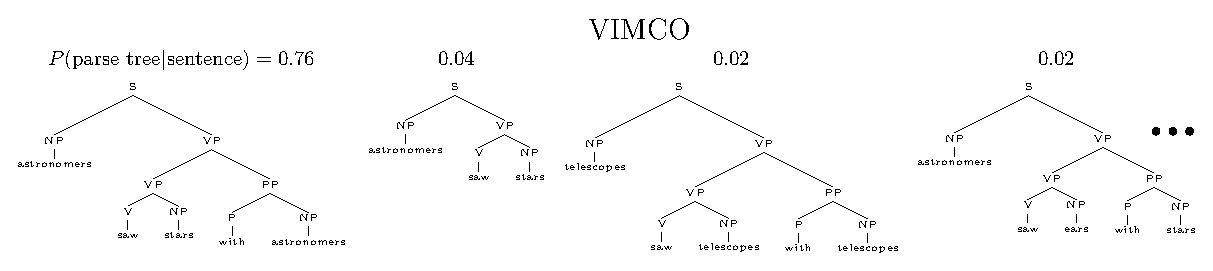
\includegraphics[width=\textwidth]{figures/pcfg/vimco.eps}
% \end{figure*}

% p(tree1 | sentence) = 0.42857142857
% p(tree2 | sentence) = 0.57142857142

\begin{figure*}[!ht]
  \includegraphics[width=0.33\textwidth]{figures/air/logp_test.pdf}
  \includegraphics[width=0.33\textwidth]{figures/air_logp_end_2.pdf}
  \includegraphics[width=0.33\textwidth]{figures/air/kl_test.pdf}
  \caption{
    Training of \gls{AIR}.
    \emph{(Left)}
    Training curves:
    % there is larger variance in models learned with \gls{VIMCO}.
    training with \gls{VIMCO} leads to larger variance in training than \gls{WW}.
    \emph{(Middle)}
    Log evidence values at the end of training:
    increasing number of particles improves \gls{WW} monotonically but improves \gls{VIMCO} only up to a point ($K = 10$ is the best).
    \emph{(Right)}
    \gls{WW} results in significantly lower variance and better inference networks than \gls{VIMCO}.
    Note that \gls{KL} is between the inference network and the \emph{current} generative model.
  }
  \label{fig:air_logp}
  \vspace*{-2ex}
\end{figure*}

\subsection{ATTEND, INFER, REPEAT}
\label{sec:experiments/air}

% model
Next, we evaluate \gls{WW} and \gls{VIMCO}
% (the best performing \gls{IWAE}-based algorithm for the \gls{GMM})
on \gls{AIR}~\citep{eslami2016attend}, a structured deep generative model with both discrete and continuous latent variables.
%
\Gls{AIR} uses the discrete variable to decide how many continuous variables are necessary to explain an image.
%
The sequential inference procedure of \gls{AIR} poses a difficult problem, since it implies a sequential decision process with possible branching.
%
See \citep{eslami2016attend} and \cref{app:air} for the model notation and details.

% training
We set the maximum number of inference steps in \gls{AIR} to three and train on $50 \times 50$ images with zero, one or two \acrshort{MNIST} digits.
%
The training and testing data sets consist of $60000$ and $10000$ images respectively, generated from the respective \acrshort{MNIST} train/test datasets.
%
Unlike \gls{AIR}, which used Gaussian likelihood with fixed standard deviation and continuous inputs (i.e., input $\mathbf{x} \in [0, 1]^{50 \times 50}$), we use a Bernoulli likelihood and binarized data; the stochastic binarization is similar to \citet{burda2016importance}.
%
% This choice is motivated by initial experiments, which have shown that the original setup is detrimental to the sleep phase of \gls{WS} -- samples from the generative model did not look similar to true data even after the training has converged.
%
Training is performed over two million iterations by RmsProp \citep{tieleman2012rms} with the learning rate of $10^{-5}$, which is divided by three after $400$k and $1000$k training iterations.
%
We set the glimpse size to $20 \times 20$.

% evaluation
We first evaluate the generative model via the average test log marginal where each log marginal is estimated by a one-sample, $5000$-particle \gls{IWAE} estimate.
%
The inference network is then evaluated via the average test \gls{KL} from the inference network to the posterior under the current model where each $\KL(q_\phi(z \given x), p_\theta(z \given x))$ is estimated as a difference between the log marginal estimate above and a $5000$-sample, one-particle \gls{IWAE} estimate.
%
Note that this estimate is just a proxy to the desired \gls{KL} from the inference network to the \emph{true} model posterior.
%
% Finally, we approximate the accuracy of number of inference steps as a proxy for the qualities of both the generative model and inference network.

% result
This experiment confirms that increasing number of particles improves \gls{VIMCO} only up to a point, whereas \gls{WW} improves monotonically with increased~\(K\) (\cref{fig:air_logp}).
%
\Gls{WW} also results in significantly lower variance and better inference networks than \gls{VIMCO}.

%%%%%%%%%%%%%%%%%%%%%%%%%%%%%%%%%%%%%%%%%%%%%%%%%%%%%%%%%%%%%%%%%%%%%%%%%%%%%%
% Run eval and restore !!!!!!!!!!!!!!!!!!!!!!!!!!!!!!!!!!
%
%
% the below num steps accuracy in AIR is importance-resampled, with different number of particles for every model (the same K as used for training); for this reason I don't think it is valid to report it as is. I think I can still evaluate it for M=100, say, and K=1 (k=1 to emphasise quality of q). For now, though, it's misleading.
%
%
%
%    \begin{table}[ht]
%      \centering
%      \caption{Accuracy of number of inference steps in \gls{AIR} is better for \gls{WW} than \gls{VIMCO}.}
%      \label{table:air_accuracy}
%      \begin{tabular}{@{}llllll@{}}
%      \toprule
%      $K$ & $5$ & $10$ & $20$ & $40$ & $80$ \\ \midrule
%      \gls{IWAE} & $0.949 \pm 0.063$ & $0.997 \pm 0.001$ & $0.997 \pm 0.000$ & $0.830 \pm 0.289$ & $0.997 \pm 0.002$ \\
%      \gls{WW}   & $0.997 \pm 0.000$ & $0.997 \pm 0.000$ & $0.997 \pm 0.000$ & $0.983 \pm 0.025$ & $0.996 \pm 0.001$ \\ \bottomrule
%      \end{tabular}
%    \end{table}
%%%%%%%%%%%%%%%%%%%%%%%%%%%%%%%%%%%%%%%%%%%%%%%%%%%%%%%%%%%%%%%%%%%%%%%%%%%

    % \begin{figure}
    %     \centering
    %     \includegraphics[width=0.5\linewidth]{air/logp_test}
    %     \caption{AIR: Marginal log likelihood. Solid lines are means and shaded regions represent one standard deviation. Standard deviation has been omitted for cases where the mean standard deviation is greater than $5$.}
    %     \label{fig:air_logp}
    % \end{figure}

    % \begin{figure}
    %     \centering
    %     \includegraphics[width=0.5\linewidth]{air/vae_test}
    %     \caption{AIR: The evidence lower-bound. Solid lines are means and shaded regions represent one standard deviation. Standard deviation has been omitted for cases where the mean standard deviation is greater than $5$.}
    %     \label{fig:air_vae}
    % \end{figure}

    % \begin{figure}
    %     \centering
    %     \includegraphics[width=0.5\linewidth]{air/kl_test}
    %     \caption{AIR: KL-divergence between the approximate posterior and the posterior of the current model. Solid lines are means and shaded regions represent one standard deviation. Standard deviation has been omitted for cases where the mean standard deviation is greater than $5$.}
    %     \label{fig:air_acc}
    % \end{figure}

    % \begin{figure}
    %     \centering
    %     \includegraphics[width=0.5\linewidth]{air/num_step_acc_test}
    %     \caption{AIR: Accuracy of number of inference steps. Solid lines are means and shaded regions represent one standard deviation. Standard deviation has been omitted for cases where the mean standard deviation is greater than $0.1$.}
    %     \label{fig:air_acc_2}
    % \end{figure}




%numbers for AIR:
%
%tag, target, k, mean+-std, mean_std_across_training
%
%vae_test
%vae_test, iwae_vimco, 80, -461.778+-194.494 214.07364
%vae_test, iwae_vimco, 40, -268.693+-234.041 196.0884
%vae_test, iwae_vimco, 20, -154.271+-43.617 19.922382
%vae_test, iwae_vimco, 10, -183.581+-80.310 38.15588
%vae_test, iwae_vimco, 5, -113.130+-9.452 7.988214
%vae_test, rw_rw, 80, -103.821+-0.086 0.27857488
%vae_test, rw_rw, 40, -104.072+-0.759 0.67278016
%vae_test, rw_rw, 20, -103.609+-0.265 0.32347438
%vae_test, rw_rw, 10, -104.129+-0.301 0.35700417
%vae_test, rw_rw, 5, -104.523+-0.252 0.3047606
%vae_test
%vae_test, iwae_vimco, 80, -461.778+-194.494 214.07364
%vae_test, iwae_vimco, 40, -268.693+-234.041 196.0884
%vae_test, iwae_vimco, 20, -154.271+-43.617 19.922382
%vae_test, iwae_vimco, 10, -183.581+-80.310 38.15588
%vae_test, iwae_vimco, 5, -113.130+-9.452 7.988214
%vae_test, rw_rw, 80, -103.821+-0.086 0.27857488
%vae_test, rw_rw, 40, -104.072+-0.759 0.67278016
%vae_test, rw_rw, 20, -103.609+-0.265 0.32347438
%vae_test, rw_rw, 10, -104.129+-0.301 0.35700417
%vae_test, rw_rw, 5, -104.523+-0.252 0.3047606
%kl_test
%kl_test, iwae_vimco, 80, 355.846+-194.526 214.1097
%kl_test, iwae_vimco, 40, 165.203+-234.058 196.11067
%kl_test, iwae_vimco, 20, 55.454+-43.618 19.963625
%kl_test, iwae_vimco, 10, 84.986+-80.311 38.194466
%kl_test, iwae_vimco, 5, 13.805+-9.457 8.035896
%kl_test, rw_rw, 80, 6.978+-0.098 0.28919804
%kl_test, rw_rw, 40, 6.818+-0.797 0.7250941
%kl_test, rw_rw, 20, 5.995+-0.267 0.32935238
%kl_test, rw_rw, 10, 5.858+-0.323 0.37547684
%kl_test, rw_rw, 5, 5.362+-0.333 0.3886485
%kl_test
%kl_test, iwae_vimco, 80, 355.846+-194.526 214.1097
%kl_test, iwae_vimco, 40, 165.203+-234.058 196.11067
%kl_test, iwae_vimco, 20, 55.454+-43.618 19.963625
%kl_test, iwae_vimco, 10, 84.986+-80.311 38.194466
%kl_test, iwae_vimco, 5, 13.805+-9.457 8.035896
%kl_test, rw_rw, 80, 6.978+-0.098 0.28919804
%kl_test, rw_rw, 40, 6.818+-0.797 0.7250941
%kl_test, rw_rw, 20, 5.995+-0.267 0.32935238
%kl_test, rw_rw, 10, 5.858+-0.323 0.37547684
%kl_test, rw_rw, 5, 5.362+-0.333 0.3886485
%logpx_test
%logpx_test, iwae_vimco, 80, -105.932+-3.512 3.614406
%logpx_test, iwae_vimco, 40, -103.490+-2.875 2.5203645
%logpx_test, iwae_vimco, 20, -98.817+-0.268 0.75712645
%logpx_test, iwae_vimco, 10, -98.595+-0.378 0.7549159
%logpx_test, iwae_vimco, 5, -99.324+-0.283 0.42569834
%logpx_test, rw_rw, 80, -96.842+-0.046 0.0680763
%logpx_test, rw_rw, 40, -97.254+-0.243 0.2675206
%logpx_test, rw_rw, 20, -97.614+-0.033 0.051102422
%logpx_test, rw_rw, 10, -98.271+-0.116 0.10897209
%logpx_test, rw_rw, 5, -99.161+-0.218 0.23595817
%
%num_steps_acc_test, iwae_vimco, 80, 0.997+-0.002 0.0097846912577274
%num_steps_acc_test, iwae_vimco, 40, 0.830+-0.289 0.24703451530470122
%num_steps_acc_test, iwae_vimco, 20, 0.997+-0.000 0.005596457855210997
%num_steps_acc_test, iwae_vimco, 10, 0.997+-0.001 0.008849094343651977
%num_steps_acc_test, iwae_vimco, 5, 0.949+-0.063 0.06692072584329027
%num_steps_acc_test, rw_rw, 80, 0.996+-0.001 0.0008066281251088672
%num_steps_acc_test, rw_rw, 40, 0.983+-0.025 0.02411366072534301
%num_steps_acc_test, rw_rw, 20, 0.997+-0.000 0.00047535752918038856
%num_steps_acc_test, rw_rw, 10, 0.997+-0.000 0.0005349459234959429
%num_steps_acc_test, rw_rw, 5, 0.997+-0.000 0.000862527605328427

% \begin{figure}
%     \centering
%     \includegraphics[width=0.5\linewidth]{air/fixed_prior_iwae_test}
%     \caption{AIR with fixed priors: \textsc{IWAE}-5 bound. \ak{This is just to show correctness of IWAE+VIMCO implementation and should be moved into appendix in case of space issues.}}
%     \label{fig:air_iwae_fixed_prior}
% \end{figure}

% \begin{figure}
%     \centering
%     \includegraphics[width=0.5\linewidth]{air/fixed_prior_vae_test}
%     \caption{AIR with fixed priors: \textsc{IWAE}-5 bound. \ak{This is just to show correctness of IWAE+VIMCO implementation and should be moved into appendix in case of space issues.}}
%     \label{fig:air_iwae_fixed_prior_2}
% \end{figure}

\subsection{GAUSSIAN MIXTURE MODEL}
\label{sec:experiments/gmm}

\begin{figure*}[!ht]
  \centering
  % \includegraphics[width=0.9\textwidth]{figures/gmm/plot_paper.pdf}
  % \includegraphics[width=0.89\textwidth]{figures/gmm/errors.pdf}
  \includegraphics[width=\textwidth]{figures/gmm/errors_no_std.pdf}
  \vspace*{-4ex}
  \caption{
    \Gls{GMM} training.
    Median and interquartile ranges from $10$ repeats shown.
    \emph{(Top)}
    Quality of the generative model:
    \gls{WS} and \gls{WW} improve with more particles thanks to lower variance and lower bias estimators of the gradient respectively.
    \Gls{IWAE} methods suffer with a larger particle budget~\citep{rainforth2018tighter}.
    \Gls{WS} performs the worst as a consequence of computing the expected \gls{KL} under the model distribution~\(p_\theta(x)\)~\cref{eq:sleep-phi-obj} instead of the true data distribution~\(p(x)\) as with \gls{WW}~\cref{eq:wake-phi-obj}.
    \Gls{WW} suffers from branch-pruning (see text) in low-particle regimes, but learns the best model fastest in the many-particle regime; $\delta$-\gls{WW} additionally learns well in the low-particle regime.
    \emph{(Bottom)}
    Both inference network and generative model quality develop identically.
    % \emph{(Bottom)}
    % \Gls{WW} and \gls{WS} have lower-variance gradient estimators of $\phi$ than \gls{IWAE}, as they avoid the high-variance term \circled{1} in \eqref{eq:iwae-reinforce}.
    % This is a necessary, but not sufficient, condition for efficient learning, with other factors being gradient direction and the ability to escape local optima.
  }
  \label{fig:gmm}
  \vspace*{-1ex}
\end{figure*}

% model
% \setlength{\columnsep}{1pt}
% \begin{wrapfigure}[7]{r}{0.21\textwidth}
%   \centering
%   \vspace*{-3ex}
%   \includegraphics[width=0.95\linewidth,trim={1em 0 1em 1em},clip]{figures/gmm_true_dist.pdf}
%   \vspace*{-2.5ex}
%   \caption{True \gls{GMM}.}
%   \label{fig:true-gmm}
% \end{wrapfigure}
%
In order to examine the differences between \gls{RWS} and \gls{IWAE} more closely, we study  a \gls{GMM} which branches on a discrete latent variable to select cluster assignments.
The generative model and inference network are defined as
%
% {\footnotesize
\begin{align*}
  p_\theta(z) &= \mathrm{Cat}(z \given \mathrm{softmax}(\theta)),\,\,
  p(x \given z) = \mathcal{N}(x \given \mu_z, \sigma_z^2), \\
  q_\phi(z \given x) &= \mathrm{Cat}(z \given \mathrm{softmax}(\eta_\phi(x))),
\end{align*}
% }
%
where $z \in \{0, \dotsc, C - 1\}$,  $C$ is the number of clusters and $\mu_c, \sigma_c^2$ are fixed to $\mu_c = 10c$ and $\sigma_c^2 = 5^2$.
The generative model parameters are $\theta \in \mathbb R^C$.
The inference network consists of a \acrlong{MLP} $\eta_\phi: \mathbb R \to \mathbb R^C$, with the $1$-$16$-$C$ architecture and the $\tanh$ nonlinearity, parameterized by $\phi$.
The chosen family of inference networks is empirically expressive enough to capture the posterior under the true model.
The true model is set to $p_{\theta_\text{true}}(x)$ where $\mathrm{softmax}(\theta_\text{true})_c = (c + 5) / \sum_{i = 1}^C (i + 5)$ ($c = 0, \dotsc, C - 1$), i.e. the mixture probabilities are linearly increasing with the $z$
.
% (\cref{fig:true-gmm}).
We fix the mixture parameters in order to study the important features of the problem at hand in isolation.

% training details
We train using \gls{WS}, \gls{WW}, as well as using \gls{IWAE} with \acrshort{REINFORCE}, \acrshort{RELAX}, \gls{VIMCO} and the Concrete distribution.
%
We attempted different variants of relaxations \citep{rolfe2016dvae,vahdat2018dvaepp} in this setting, but they performed considerably worse than any of the alternatives (c.f. \Cref{app:dvae}).
%
We fix $C = 20$ and increase number of particles from $K = 2$ to $20$.
%
We use the Adam optimizer with default parameters.
%
Each training iteration samples a batch of $100$ data points from the true model.
%
Having searched over several temperature schedules for the Concrete distribution, we use the one with the lowest trainable terminal temperature (linearly annealing from $3$ to $0.5$).
%
We found that using the control variate $c_\rho(g_{1:K}) = \frac{1}{K} \sum_{k = 1}^K \acrshort{MLP}_\rho([x, g_k])$, with \gls{MLP} architecture $(1 + C)$-$16$-$16$-$1$ ($\tanh$) led to most stable training (c.f.\ \cref{app:gmm}).

% evaluation details
% We evaluate the generative model, inference network.
The generative model is evaluated via the $L_2$ distance between the \glspl{PMF} of its prior and true prior as $\|\mathrm{softmax}(\theta) - \mathrm{softmax}(\theta_\text{true})\|$.
The inference network is evaluated via the $L_2$ distance between \glspl{PMF} of the current and true posteriors, averaged over a fixed set~(\(M=100\)) of observations $(x_{\text{test}}^{(m)})_{m = 1}^{M}$ from the true model: $\frac{1}{M} \sum_{m = 1}^M \|q_\phi(z \given x_{\text{test}}^{(m)}) - p_{\theta_{\text{true}}}(z \given x_{\text{test}}^{(m)})\|$.
% Finally, \(\phi\)'s gradient-estimator standard deviation is given by $\frac{1}{D_\phi} \sum_{d = 1}^{D_\phi} \std(g_d)$ where $g_d$ is the $d$th (out of $D_\phi$) element of one of~\(\phi\)'s gradient estimators (e.g. \cref{eq:iwae-reinforce} for \acrshort{REINFORCE}) and $\std(\cdot)$ is estimated using $10$ samples.

% results & zero forcing & defensive IS
% Here, we demonstrate that increasing number of particles leads to better inference networks for \gls{WS} and \gls{WW} but not for \gls{IWAE} methods (\cref{fig:gmm}, Middle).
We demonstrate that using \gls{WS} and \gls{WW} with larger particle budgets leads to better inference networks whereas this is not the case for \gls{IWAE} methods (\cref{fig:gmm}, bottom).
% Here, we demonstrate that using \gls{WS} and \gls{WW} leads to a better inference networks when number of particles is increased whereas this is not the case for \gls{IWAE} methods (\cref{fig:gmm}, Middle).
Recall that the former is because using more samples to estimate the gradient of the sleep $\phi$ objective \cref{eq:sleep-phi-obj} for \gls{WS} reduces variance at a standard Monte Carlo rate and that using more particles in \cref{eq:wake-phi-est} to estimate the gradient of the wake $\phi$ objective results in a lower bias.
The latter is because using more particles results in the signal-to-noise of \gls{IWAE}'s $\phi$ gradient estimator to drop at the rate $O(1 / \sqrt{K})$~\citep{rainforth2018tighter}.

Learning of the generative model, through inference-network learning, also monotonically improves with increasing \(K\) for \gls{WS} and \gls{WW}, but worsens for all \gls{IWAE} methods except \gls{VIMCO}, since the $\theta$ gradient estimator (common to all methods), $\nabla_\theta \ELBO_{\acrshort{IS}}^K(\theta, \phi, x)$ can be seen as an importance sampling estimator whose quality is tied to the proposal distribution (inference network).

To highlight the difference between \gls{WW} and \gls{WS}, we study the performance of the generative model and the inference network for different initializations of $\theta$.
In \cref{fig:gmm}, $\theta$ is initialized such that the mixture probabilities are exponentially decreasing with $z$ which results in the data distribution $p_\theta(x)$ being far from $p_{\theta^*}(x)$.
Consequently, the sleep-phase $\phi$ update is highly biased which is supported by \gls{WS} being worse than \gls{WW}.
On the other hand, if $\theta$ is initialized such that the mixture probabilities are equal, $p_\theta(x)$ is closer to $p_{\theta^*}(x)$, which is supported by \gls{WS} outperforming \gls{WW} (see \cref{app:gmm/additional}).

% \Gls{WW} and \gls{WS} have lower variance gradient estimators than \gls{IWAE}, even if used with control-variate and continuous-relaxation methods.
% %
% This is because $\phi$'s gradient estimators for \gls{WW} and \gls{WS} do not include the high-variance term \circled{1} in \cref{eq:iwae-reinforce}.
% %
% This is a necessary but not sufficient condition for efficient learning with other important factors being gradient direction and the ability to escape local optima (explored below).
% %
% Employing the Concrete distribution gives low-variance gradients for $\phi$ to begin with, but the model learns poorly due to the high gradients bias (due to high temperature hyperparameter).

\begin{figure*}[!ht]
  \centering
  % \includegraphics[width=\textwidth]{figures/gmm/plot_paper_2.pdf}
  % \includegraphics[width=\textwidth]{figures/gmm/plot_paper_2_stair.pdf}
  % \includegraphics[width=0.9\textwidth]{figures/gmm/plot_paper_3.pdf}
  \includegraphics[width=\textwidth]{figures/gmm/models.pdf}
  \vspace*{-4ex}
  \caption{
    Generative model and inference network during \gls{GMM} training shown as Hinton diagrams where areas are proportional to probability.
    % $z$ goes from $0$ to $19$, left to right.
    Rows correspond to start, middle and end of optimization.
    \emph{(Left half)}
    Learning with few particles leads to the branch-pruning (described in text) of the inference network (shown as conditional \gls{PMF} given different $x$) and the generative model (first column of each half) for all methods except $\delta$-\gls{WW}.
    Concrete distribution fails.
    \emph{(Right half)}
    Learning with many particles leads to branch-pruning only for \gls{WS}; \gls{WW} and $\delta$-\gls{WW} succeed where \gls{IWAE} fails, learning a suboptimal final generative model.
  }
  \label{fig:gmm2}
\end{figure*}

We now describe a failure mode affecting \gls{WS}, \gls{WW}, \gls{VIMCO}, \acrshort{RELAX} and \acrshort{REINFORCE} due the adverse initialization of $\theta$ which we call \emph{branch-pruning}.
%
It is best illustrated by inspecting the generative model and the inference network as training progresses, focusing on the low-particle ($K = 2$) regime (\cref{fig:gmm2}).
%
For \gls{WS}, the generative model $p_\theta(z)$ peaks at $z = 9$ and puts zero mass for $z > 9$; the inference network $q_\phi(z \given x)$ becomes the posterior for this model which, here, has support at most $\{0, \dotsc, 9\}$ for all $x$.
% is a delta mass at $z = 9$ for $x$ larger than around $90$ ($x = 95$ and $x = 190$ shown) and a distribution with the support $\{0, \dotsc, 9\}$ for other values of $x$.
This is a local optimum for \gls{WS} as
%
\begin{inparaenum}[(i)]
\item the inference network already approximates the posterior of the model $p_\theta(z, x)$ well, and
\item the generative model $p_\theta(z)$, trained using samples from $q_\phi(z \given x)$, has no samples outside of its current support. % ($\{0, \dotsc, 9\}$).
\end{inparaenum}
%
Similar failures occur for \gls{WW} and \gls{VIMCO}/\acrshort{RELAX}/\acrshort{REINFORCE} although the support of the locally optimal $p_\theta(z)$ is larger ($\{0, \dotsc, 14\}$ and $\{0, \dotsc, 17\}$ respectively).

While this failure mode is a particular feature of the adverse initialization of $\theta$, we hypothesize that \gls{WS} and \gls{WW} suffer from it more, as they alternate between two different objectives for optimizing $\theta$ and $\phi$.
\Gls{WS} attempts to amortize inference for the current model distribution $p_\theta(x)$ which reinforces the coupling between the generative model and the inference network, making it easier to get stuck in a local optimum.
\Gls{WW} with few particles (say $K = 1$) on the other hand, results in a highly-biased gradient estimator \cref{eq:wake-phi-est} that samples $z$ from $q_\phi(\cdot \given x)$ and evaluates $\nabla_\phi \log q_\phi(z \given x)$; this encourages the inference network to concentrate mass.
This behavior is not seen in \gls{WW} with many particles where it is the best algorithm at learning both a good generative model and inference network (\cref{fig:gmm}; \cref{fig:gmm2}, right).

% Recall that \gls{WW} and \gls{WS} alternate between two different objectives for optimizing $\theta$ and $\phi$; this can lead to the optimization process getting stuck in a local optimum which prevents effective learning, especially in cases with low-dimensional latent spaces such as our \gls{GMM}.
% In this experiment, we find that using \acrshort{WW} can lead to mode collapse of the inference network in low-particle regimes (\cref{fig:gmm2}).

We propose a simple extension of \gls{WW}, denoted $\delta$-\acrshort{WW}, that mitigates this shortcoming by changing the proposal of the self-normalized importance sampling estimator in \cref{eq:wake-phi-est} to \(q_{\phi, \delta}(z \given x) = (1 - \delta) q_\phi(z \given x) + \delta \mathrm{Uniform}(z)\).
We use $\delta = 0.2$, noting that the method is robust to a range of values.
Using a different proposal than the inference network $q_\phi(z \given x)$ means that using the low-particle estimator in \cref{eq:wake-phi-est} no longer leads to branch-pruning.
This is known as defensive \acrlong{IS}~\citep{hesterberg1995weighted}, and is used to better estimate integrands that have long tails using short-tailed proposals.
Using $\delta$-\gls{WW} outperforms all other algorithms in learning both the generative model and the inference network in the low-$K$ regime and performs similarly as \gls{WW} in the high-$K$ regime.


%%% Local Variables:
%%% mode: latex
%%% TeX-master: "main"
%%% End:
%  LocalWords:  IWAE RWS sigmoid variates ELBO PCFG SCFM GMM WS VIMCO
%  LocalWords:  Notationally interquartile combinatorially infeasible
%  LocalWords:  chen dempster lari earley klein datasets SGD le RNN
%  LocalWords:  Levenshtein sisson kingma adam hyperparameters eslami
%  LocalWords:  MNIST binarized binarization burda RmsProp tieleman
%  LocalWords:  rms rainforth MLP nonlinearity parameterized softmax
%  LocalWords:  rolfe dvae vahdat dvaepp PMF initializations
%  LocalWords:  suboptimal hesterberg integrands
